\section{Tuesday, March 5th}
\subsection{Logistics}
Proposal is no longer due this Thursday, now due next Tuesday. 

A lot of students are doing the discussion only just before classes. At least once reply must be posted before (midnight on Saturday).

\subsection{Goals for the week:}
\begin{enumerate}
    \item Week 7 (Information) Review
    \item Information Geometry
    \begin{itemize}
        \item Example on Maximum Geometry
    \end{itemize}
\end{enumerate}
\subsubsection{Challenge for the week:}
\begin{important}
\textbf{Challenge:} Use Maximum Geometry to prove the \textit{Central Limit Theorem}.
\end{important}

\subsection{Review of last week:}
If we have $\{X_i\}_{i=1}^n\simiid p$ where $p = p_0$ or $p_1$.

\begin{align*}
S &= s(X_1, \ldots, X_n) = \log\left(\frac{\P[X_1, \ldots, X_n \mid p_1]}{\P[X_1, \ldots, X_n \mid p_0]}\right)
\end{align*}
\begin{important}
Note for quiz 4: The order for entries in a KL divergence do matter. You will be tested on this order. The one that goes first is the one you are drawing from:
\begin{equation}
    \E_{X\sim p_1}[S] = n D(p_1||p_0)
\end{equation}

\begin{equation}
    \E_{X\sim p_0}[S] = -n D(p_0||p_1)
\end{equation}
\end{important}
\begin{center}
    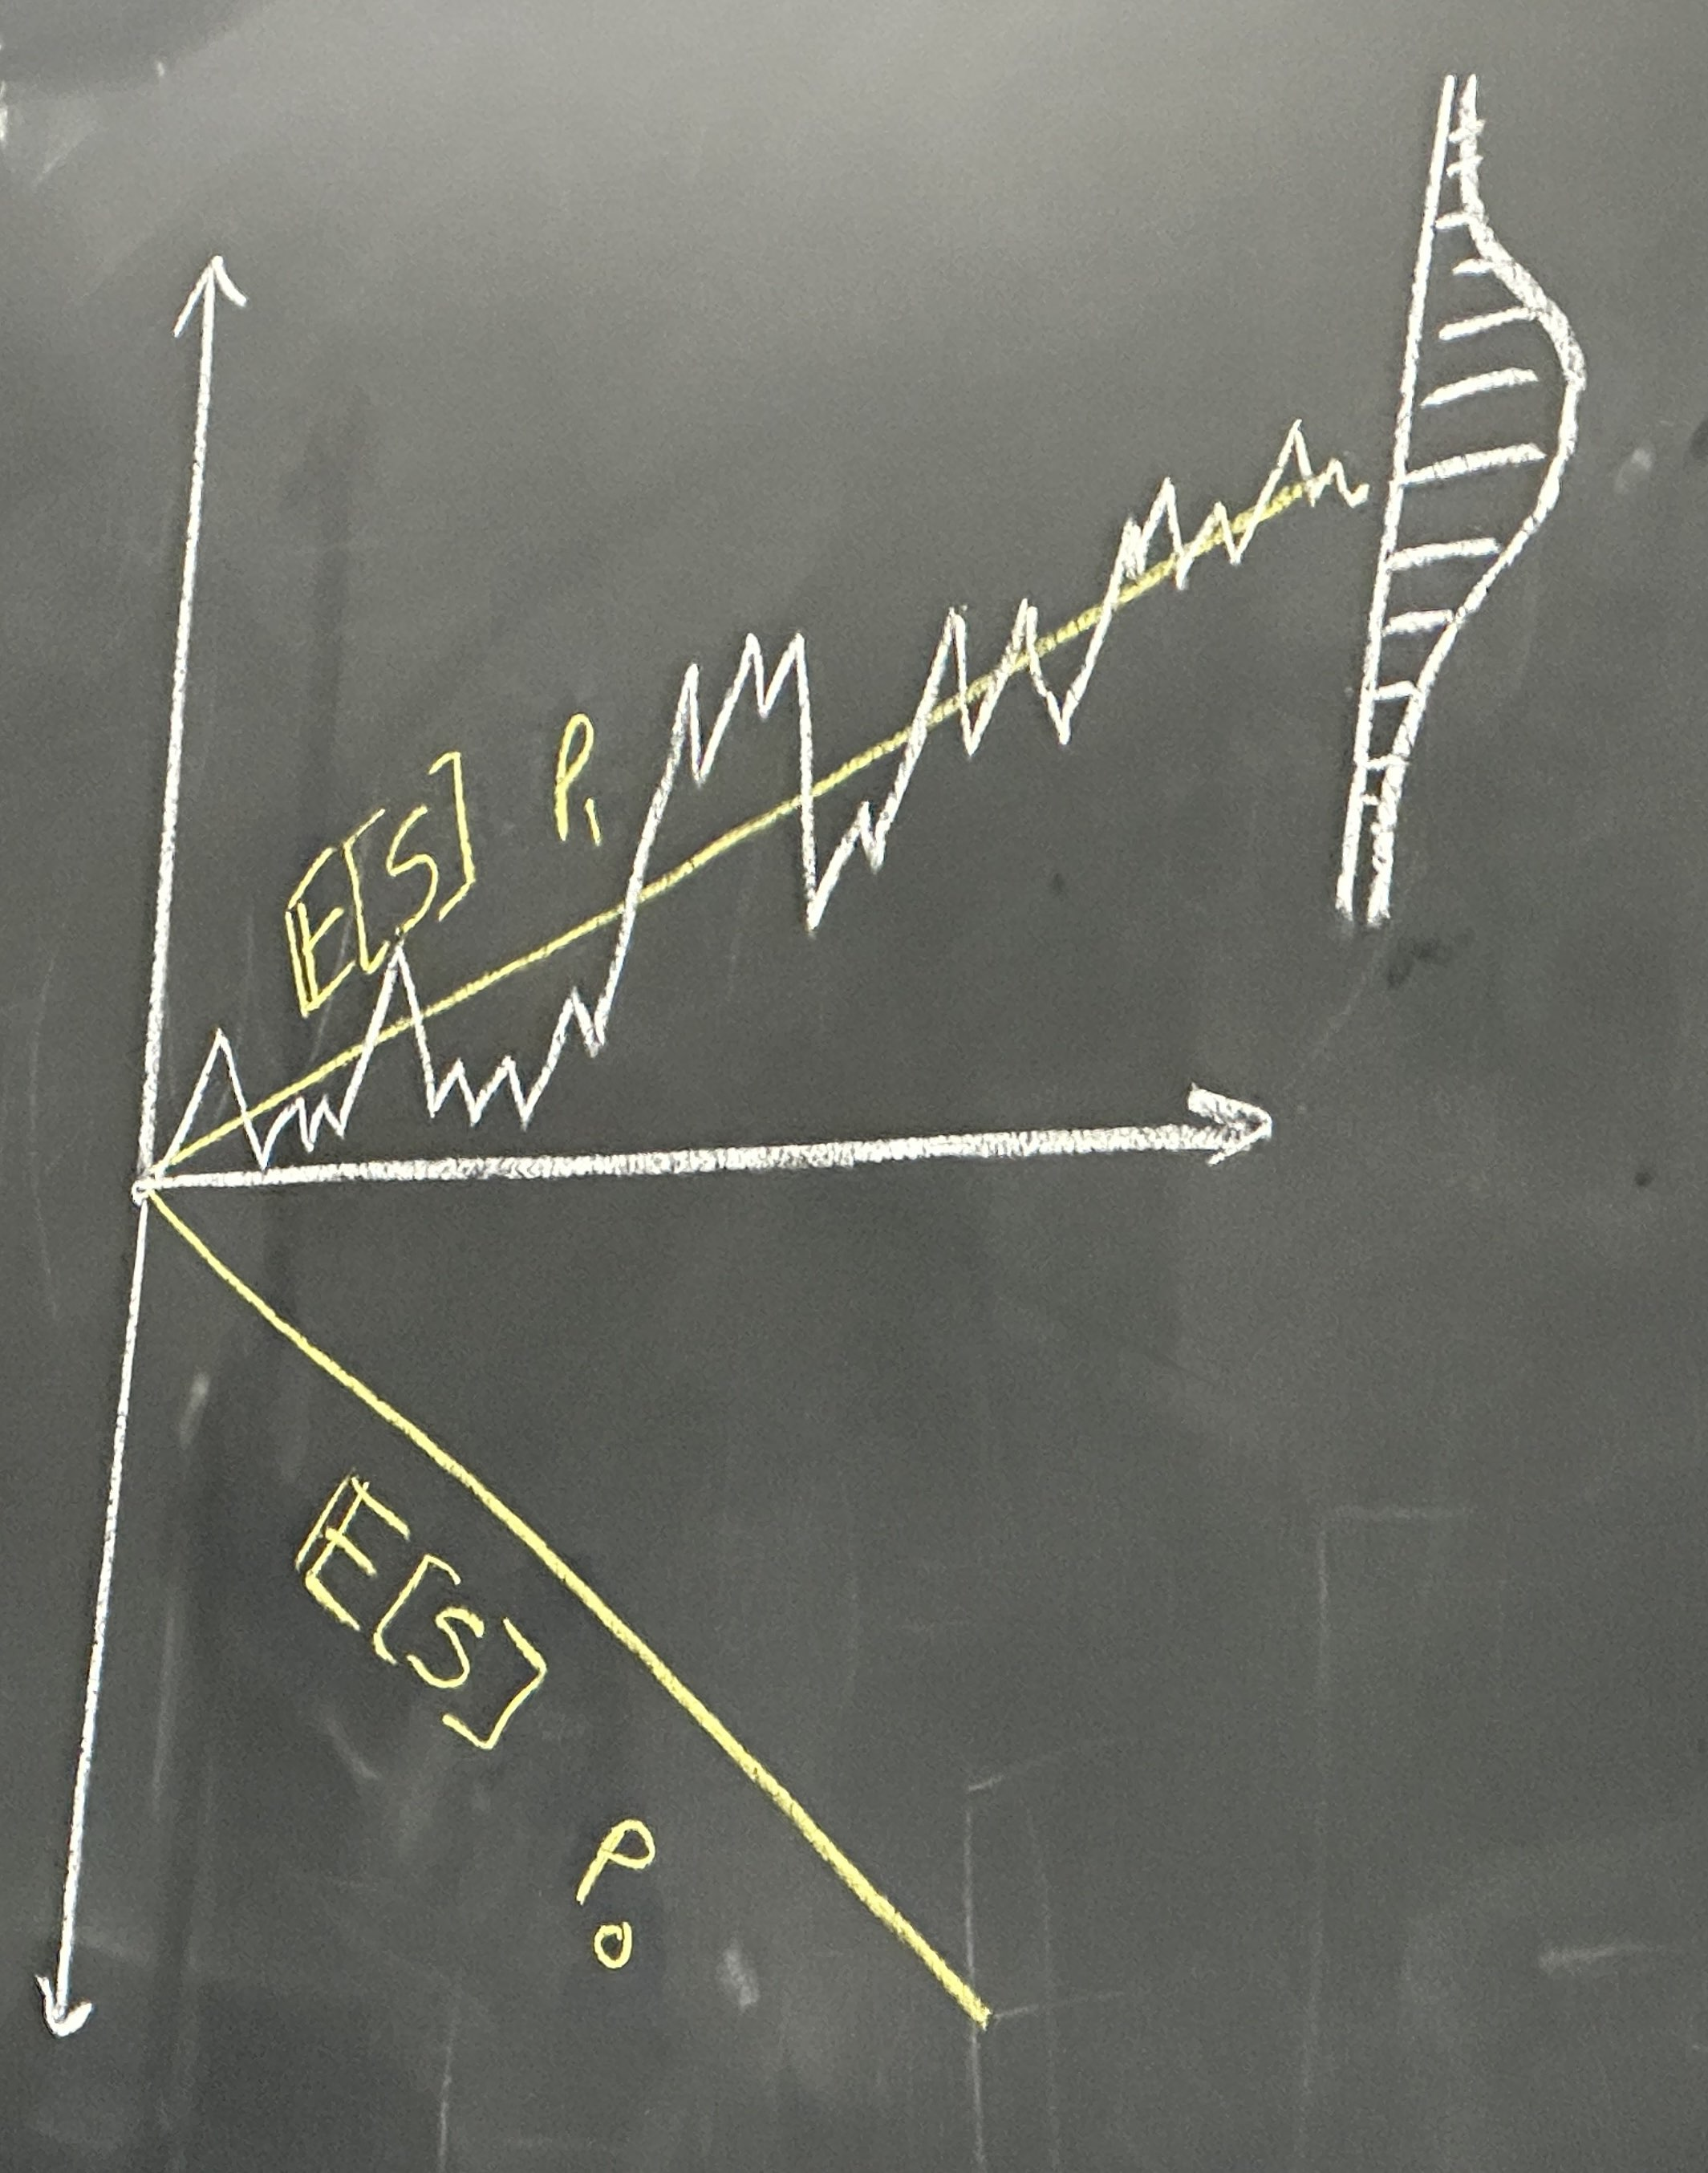
\includegraphics[scale=0.1]{lectures/wk8/img/img1.jpeg}
\end{center}
Note that $D$ controls the slope: increasing it (a change in $D$) tells you that it will be more clearly distinguishable.

Vertical distribution = background sampling distribution.

\subsection{Brownian Bridge}
\begin{center}
    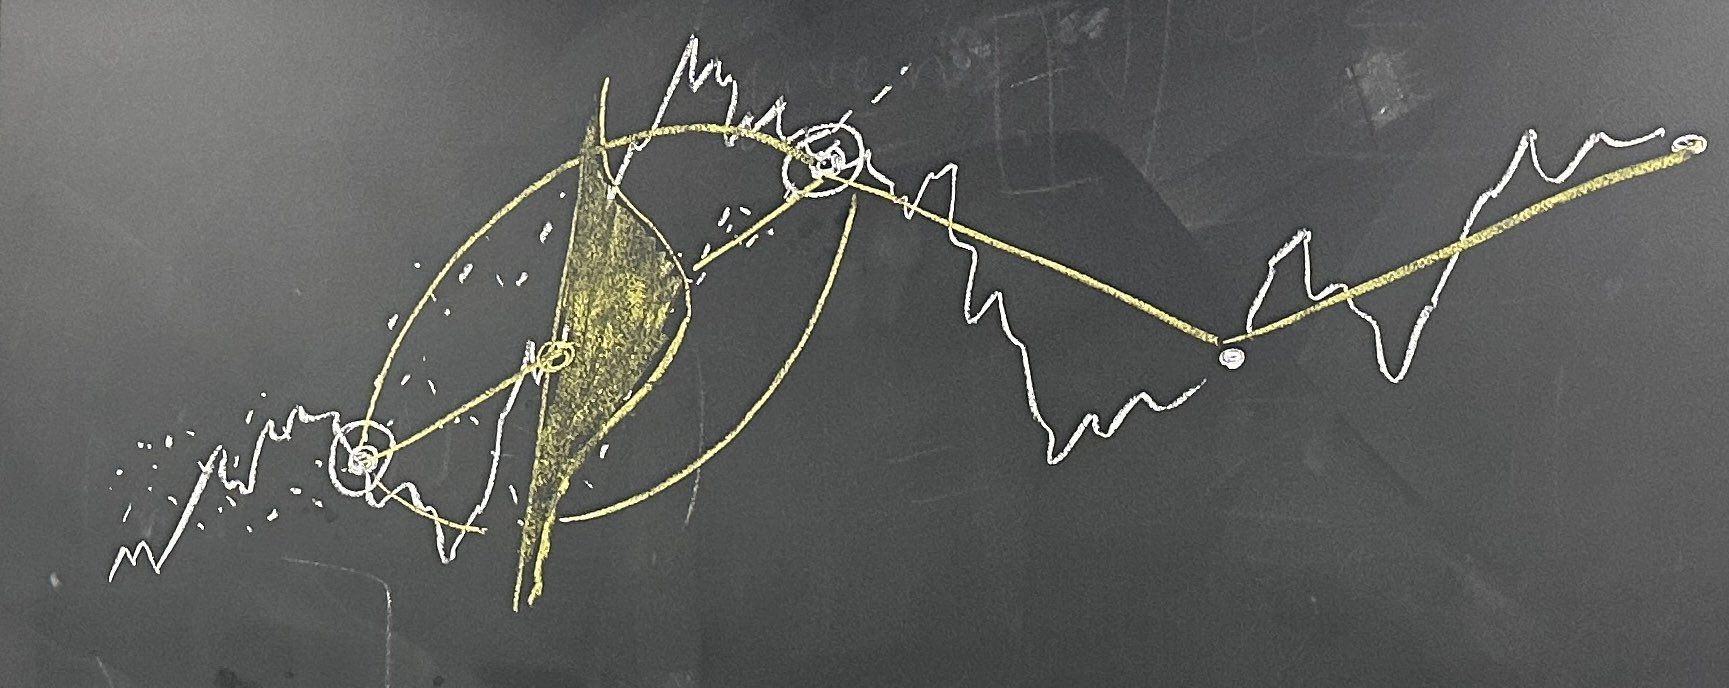
\includegraphics[scale=0.25]{lectures/wk8/img/img2.jpeg}
\end{center}

\subsection{Problem:}
\begin{enumerate}
    \item Target distribution $p_0$
    \item Chosen divergence $D$
    \item Variational family of distribution $\cP = \{\text{ set of dist. }\}$
    \begin{enumerate}
        \item[(i)] \underline{implicit}: via constraints
        \item[(i)] \underline{explicit}: via parameterized model $\{P_\Theta\}_{\text{all }\Theta}$
    \end{enumerate}
\end{enumerate}
Goal: minimize $D(p||p_0), D(p_0||p)$ given: $p\in\cP$. 

The class of F-divergences is convex, so it can be formulated as a convex optimization problem in most cases. 

\subsubsection{Variational Calculus}
Note that you will need to use variational calculus instead of regular calculus in some choices of divergence (see the book for examples on this).

\subsubsection{Fréchet derivatives}
The derivative defined on normed spaces.

\subsubsection{3D Probability Simplex}
Within this set is our target -- note that any point in the set is a distribution. 

\begin{center}
    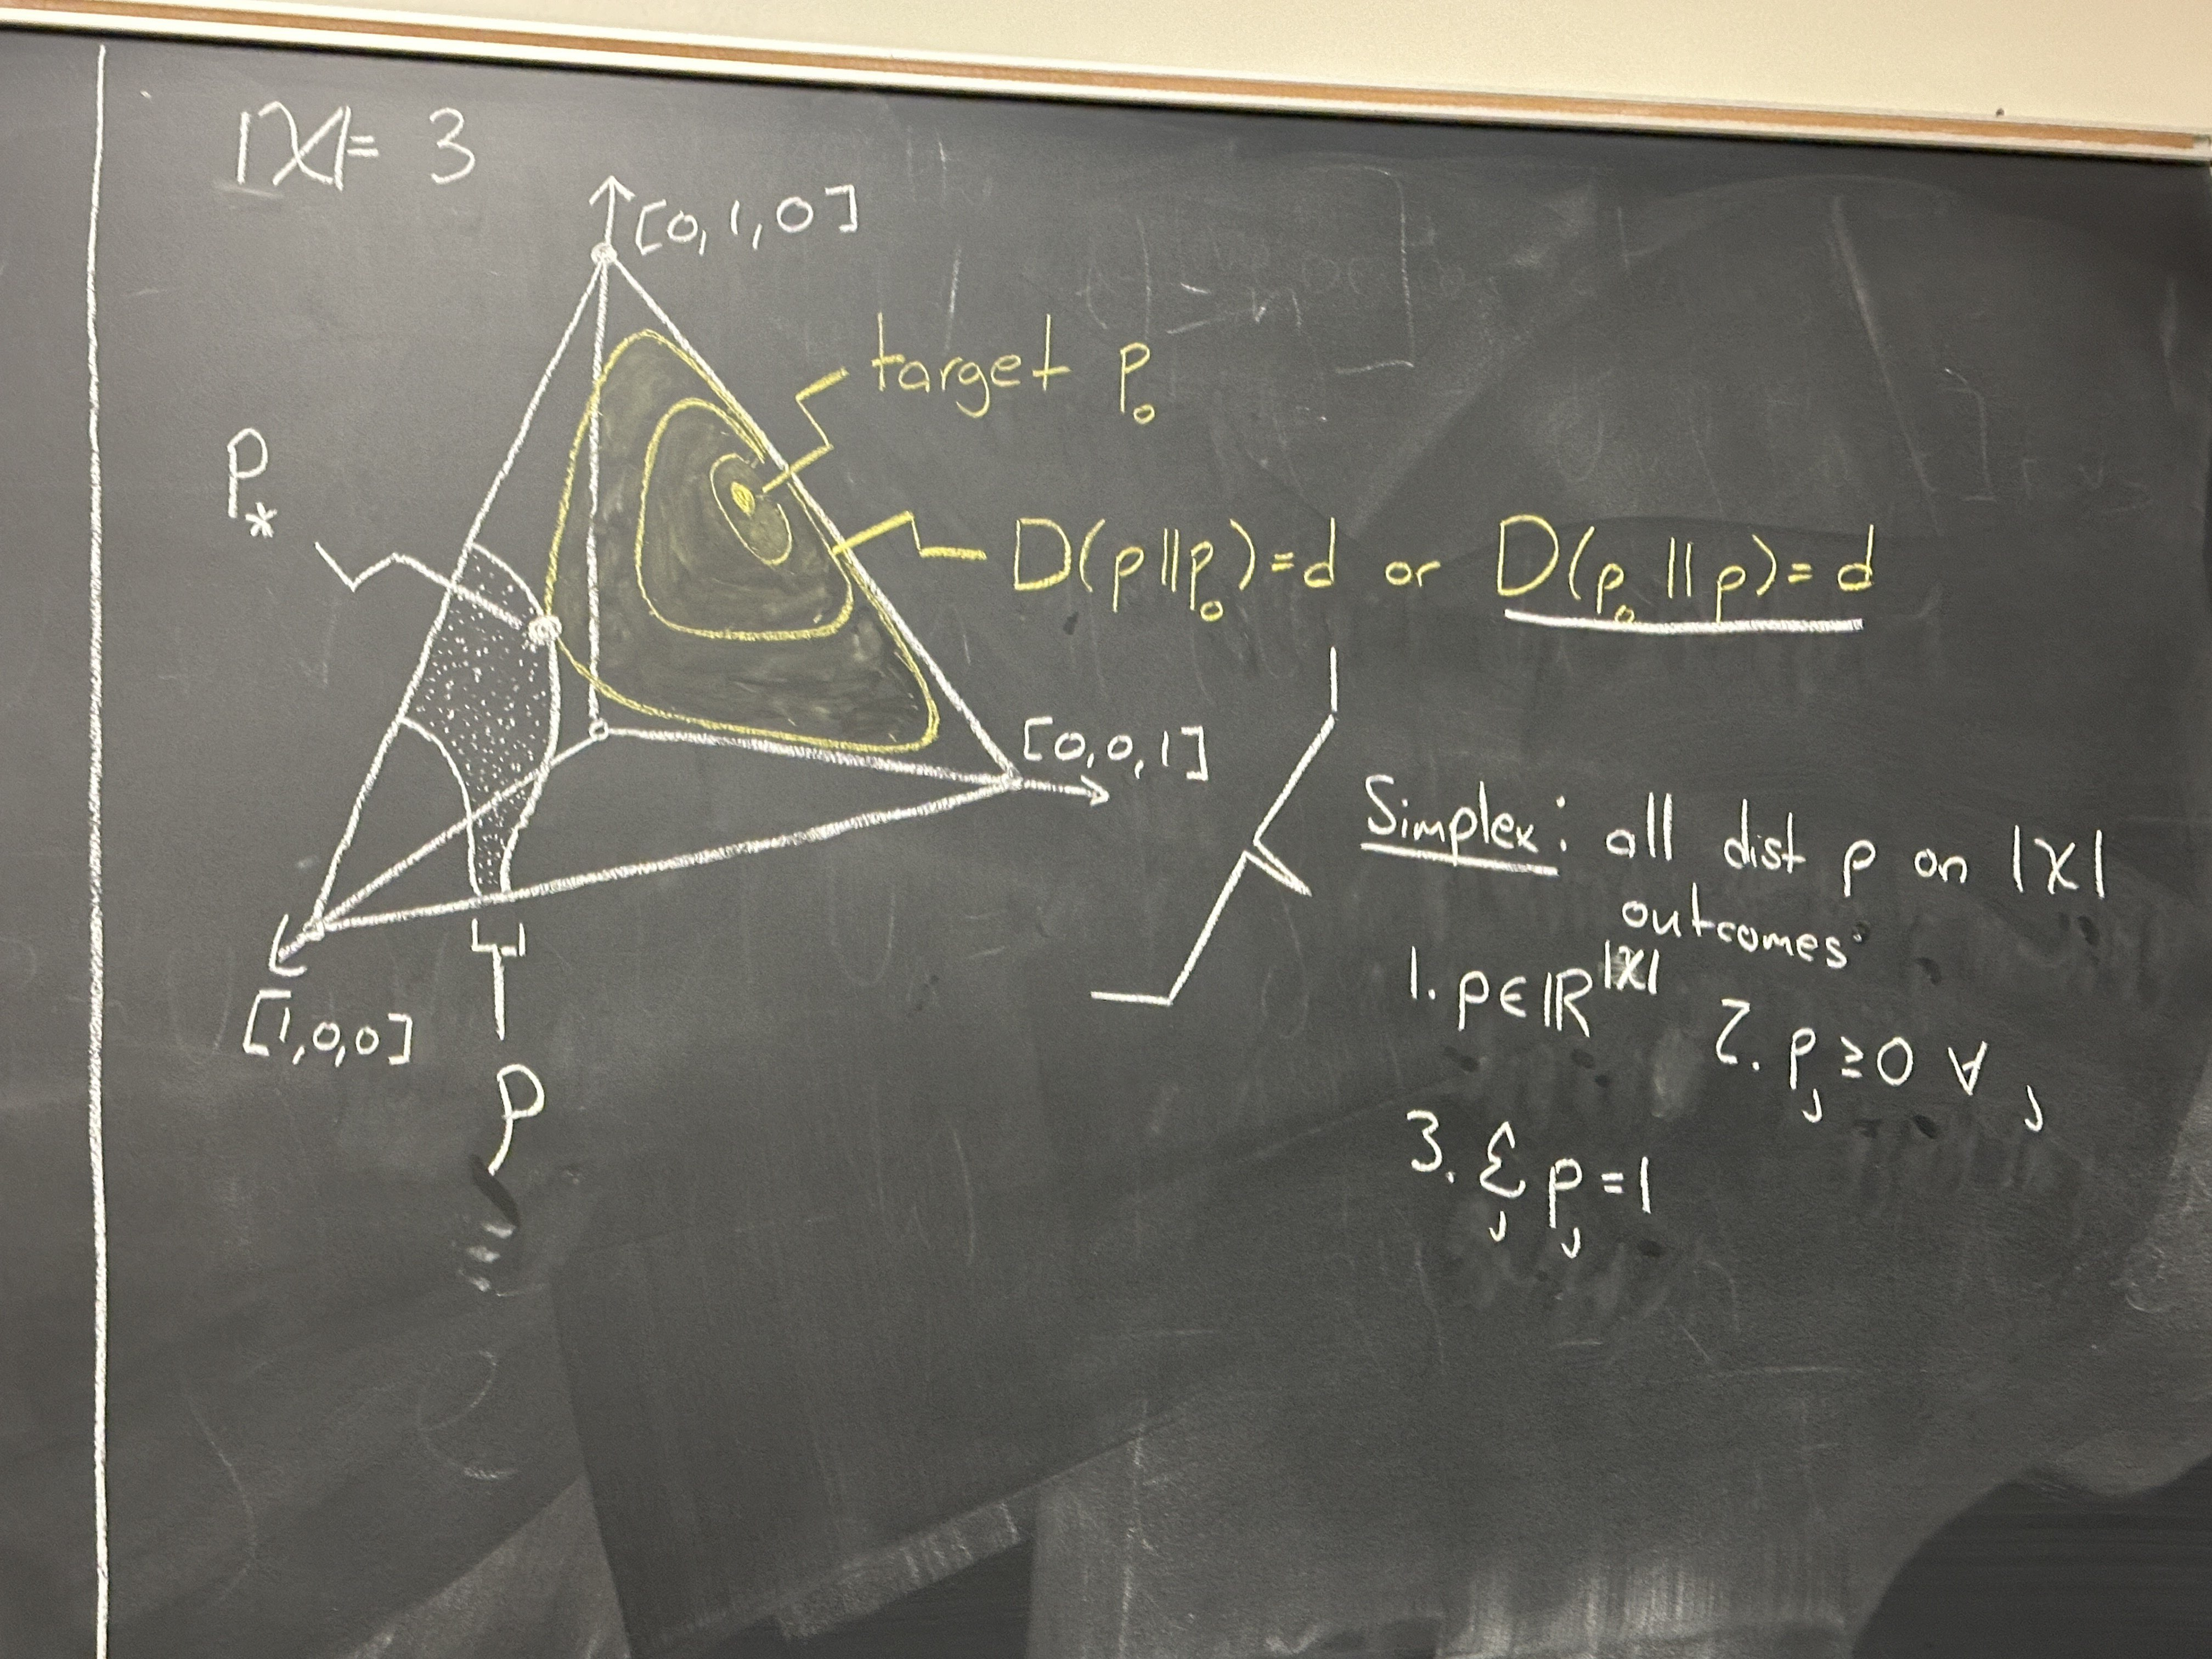
\includegraphics[scale=0.1]{lectures/wk8/img/img3.jpeg}
\end{center}

We look at the level sets that have distance $d$ away from our target $p_0$.

\subsection{Convergence in distribution on a Weak Topology}
$\underbrace{D_{KL}(p_0 || p)}_{\to0} \geq\frac1{\ln2} \underbrace{\text{TV}(p, p_0)^2}_{0} \to p \Rightarrow p_0$ which is weak convergence, 
where $\text{TV}$ is the total variation distance.

\subsection{Maximum Entropy: A constrained optimization problem}
$X\sim p$, where $p$ is unknown, but we do ``know'' some moments.

We implicitly define $\cP$ as follows:
\subsubsection{Equality:}
\underline{Equality} $\cF_i[p] = \E_{X\sim p}[f_i(x)]=\{\alpha_i\}_{i=1}^n$.

Examples:
\begin{align*}
      \E[X],& f(x) = x \\
    \E[X^2],& f(x) = x^2 \\
    &\vdots
\end{align*}


\subsubsection{Inequality:}
\underline{Inequality} $\cG_i[p] = \E_{X\sim p}[g_j(x)]\geq\{\alpha_j\}_{j=1}^m$.

\subsubsection{Goal}
We want to $\max H(p), \quad p\in\cP\implies p_\ast = 
\displaystyle\argmax_{p\in\cP} \{H(p)\}$.

\subsection{Question:}
\begin{equation}
    \max_{p\in\cP} \{H(p)\} \iff \min_{p\in\cP} \{D(? || ?)\}?
\end{equation}
\begin{important}
Quiz: You want to relate the above to the KL divergence of a uniform distribution.
\end{important}
\begin{align*}
    H(p) &= -\E_{x\sim p}[\log(p(x))]
    = -\E_{x\sim p}[\log(\frac{p(x)}{1/|\cX|} \cdot \frac1{|\cX|})]
    \\
    &= -\E_{x\sim p}[\log(\frac{p(x)}{1/|\cX|})] + \E_{x\sim p}[\log(|\cX|)] \\
    &= -D(p||U[\cX]) + H[U[\cX]] \\
H(p) &= H(U(\cX)) - D(p || U[\cX]) \\
\implies &\max_{p\in\cP} \{H(p)\} \iff \underbrace{\min_{p\in\cP} \{D(p || U[\cX])\}}_{\text{Occam's Razor for $\max H$}}
\end{align*}

\subsection{Karush-Kuhn-Tucker (KKT) Conditions:}
For Convex differentiable functions, how do we find sufficeient and necessary stationary conditions? How do we generalize Lagrange multipliers for when we have inequality constraints?

Given $\cP = \left\{p\st \underbrace{\{\cF_i[p]=\alpha_i\}_{i=1}^n}_{\text{equality}}, \underbrace{\{\cG_j[p]=\alpha_j\}_{j=1}^n}_{\text{inequality}} \right\}$

For an objective: $H(p)$
\begin{enumerate}
    \item $\left.-\nabla_p H(p) + \sum_{i=1}^n \lambda_i \nabla_p \cF(p) + \sum_{j=1}^n \mu_j \nabla_p \cG(p)\right|_{p=p^\ast}=0$
    \item $p^\ast\in\cP$
    \item $\mu_j\geq0\quad\forall j$
    \item if $G_j[p] \gneq \beta_j$ then $\mu_j=0$.
\end{enumerate}

\underline{moment:} $\cF[p] = \E_{x\sim p}[f(x)] = \sum_{\text{all $x$}} p(x) f(x)$

We are restricted to a polytope, that is a subset of a face on the simplex. 

The constraints listed above are called:

0th order optimality condition: $\forall x, p(x)\geq 0\mapsto p(x')=\begin{cases}
    0 \quad \text{ if } x'\ne x
    \\
    1 \quad \text{ if } x' = x
\end{cases}$.
\begin{enumerate}
    \item Stationarity (first order optimality condition): 
    $\sum_x p(x)=1
    \mapsto\partial_{p(x)} \sum_{x'} p(x')=1$.
    \item Feasibility (Primal), it has to live inside the set of possible distributions.
    \item Feasibility (Dual): Non-negativity, your gradient should be pointed out (not into) your set.
    \item Complementary Slackness (Active/Inactive): $\lambda_i^* h_i\left(x^*\right)=0, \forall i\quad \iff \sum()$.
\end{enumerate}

The gradient of our objective function must be parallel to the gradient of our constraints.

\subsection{Taking Derivatives:}
\begin{align*}
H(p)
&\mapsto -\partial_{p(x)} \E_{x\sim p}[\log(p(x))]  \\
&= -\partial_{p(x)} \sum_{x'}[p(x') \log(p(x'))]  \\
&= -\partial_{p(x)} [p(x) \log(p(x))]  \\
&= -\log(p(x)) - 1 \\
&= -(\log(p(x)) + 1)
\end{align*}





If the normal distribution maximizes entropy for a known mean and variance, since it is capped above by a gaussian's    .

Convergence in KL is convergence in distribution.
